%%%%%%%%%%%%%%%%%%%%%%%%%%%%%%%%%%%%%%%%%%%%%%%%%%
%  JASA LaTeX Template File
%  To make articles using JASA.cls, Version 1.1
%  September 14, 2019
%%%%%%%%%%%%%%%%%%%%%%%%%%%%%%%%%%%%%%%%%%%%%%%%%%

%% Step 1:
%% Uncomment the style that you want to use:

%%%%%%% For Preprint
%% For manuscript, 12pt, one column style

\documentclass[preprint]{JASA}

%%%%% Preprint Options %%%%%
%% The track changes option allows you to mark changes
%% and will produce a list of changes, their line number
%% and page number at the end of the article.
%\documentclass[preprint,trackchanges]{JASA}


%% NumberedRefs is used for numbered bibliography and citations.
%% Default is Author-Year style.
%% \documentclass[preprint,NumberedRefs]{JASA}

%%%%%%% For Reprint
%% For appearance of finished article; 2 columns, 10 pt fonts

% \documentclass[reprint]{JASA}

%%%%% Reprint Options %%%%%

%% For testing to see if author has exceeded page length request, use 12pt option
%\documentclass[reprint,12pt]{JASA}


%% NumberedRefs is used for numbered bibliography and citations.
%% Default is Author-Year style.
% \documentclass[reprint,NumberedRefs]{JASA}

%% TurnOnLineNumbers
%% Make lines be numbered in reprint style:
% \documentclass[reprint,TurnOnLineNumbers]{JASA}

\usepackage{natbib}


% Pandoc syntax highlighting
\usepackage{color}
\usepackage{fancyvrb}
\newcommand{\VerbBar}{|}
\newcommand{\VERB}{\Verb[commandchars=\\\{\}]}
\DefineVerbatimEnvironment{Highlighting}{Verbatim}{commandchars=\\\{\}}
% Add ',fontsize=\small' for more characters per line
\usepackage{framed}
\definecolor{shadecolor}{RGB}{248,248,248}
\newenvironment{Shaded}{\begin{snugshade}}{\end{snugshade}}
\newcommand{\AlertTok}[1]{\textcolor[rgb]{0.94,0.16,0.16}{#1}}
\newcommand{\AnnotationTok}[1]{\textcolor[rgb]{0.56,0.35,0.01}{\textbf{\textit{#1}}}}
\newcommand{\AttributeTok}[1]{\textcolor[rgb]{0.77,0.63,0.00}{#1}}
\newcommand{\BaseNTok}[1]{\textcolor[rgb]{0.00,0.00,0.81}{#1}}
\newcommand{\BuiltInTok}[1]{#1}
\newcommand{\CharTok}[1]{\textcolor[rgb]{0.31,0.60,0.02}{#1}}
\newcommand{\CommentTok}[1]{\textcolor[rgb]{0.56,0.35,0.01}{\textit{#1}}}
\newcommand{\CommentVarTok}[1]{\textcolor[rgb]{0.56,0.35,0.01}{\textbf{\textit{#1}}}}
\newcommand{\ConstantTok}[1]{\textcolor[rgb]{0.00,0.00,0.00}{#1}}
\newcommand{\ControlFlowTok}[1]{\textcolor[rgb]{0.13,0.29,0.53}{\textbf{#1}}}
\newcommand{\DataTypeTok}[1]{\textcolor[rgb]{0.13,0.29,0.53}{#1}}
\newcommand{\DecValTok}[1]{\textcolor[rgb]{0.00,0.00,0.81}{#1}}
\newcommand{\DocumentationTok}[1]{\textcolor[rgb]{0.56,0.35,0.01}{\textbf{\textit{#1}}}}
\newcommand{\ErrorTok}[1]{\textcolor[rgb]{0.64,0.00,0.00}{\textbf{#1}}}
\newcommand{\ExtensionTok}[1]{#1}
\newcommand{\FloatTok}[1]{\textcolor[rgb]{0.00,0.00,0.81}{#1}}
\newcommand{\FunctionTok}[1]{\textcolor[rgb]{0.00,0.00,0.00}{#1}}
\newcommand{\ImportTok}[1]{#1}
\newcommand{\InformationTok}[1]{\textcolor[rgb]{0.56,0.35,0.01}{\textbf{\textit{#1}}}}
\newcommand{\KeywordTok}[1]{\textcolor[rgb]{0.13,0.29,0.53}{\textbf{#1}}}
\newcommand{\NormalTok}[1]{#1}
\newcommand{\OperatorTok}[1]{\textcolor[rgb]{0.81,0.36,0.00}{\textbf{#1}}}
\newcommand{\OtherTok}[1]{\textcolor[rgb]{0.56,0.35,0.01}{#1}}
\newcommand{\PreprocessorTok}[1]{\textcolor[rgb]{0.56,0.35,0.01}{\textit{#1}}}
\newcommand{\RegionMarkerTok}[1]{#1}
\newcommand{\SpecialCharTok}[1]{\textcolor[rgb]{0.00,0.00,0.00}{#1}}
\newcommand{\SpecialStringTok}[1]{\textcolor[rgb]{0.31,0.60,0.02}{#1}}
\newcommand{\StringTok}[1]{\textcolor[rgb]{0.31,0.60,0.02}{#1}}
\newcommand{\VariableTok}[1]{\textcolor[rgb]{0.00,0.00,0.00}{#1}}
\newcommand{\VerbatimStringTok}[1]{\textcolor[rgb]{0.31,0.60,0.02}{#1}}
\newcommand{\WarningTok}[1]{\textcolor[rgb]{0.56,0.35,0.01}{\textbf{\textit{#1}}}}

% tightlist command for lists without linebreak
\providecommand{\tightlist}{%
  \setlength{\itemsep}{0pt}\setlength{\parskip}{0pt}}





\begin{document}
%% the square bracket argument will send term to running head in
%% preprint, or running foot in reprint style.

\title[A subtitle goes on another line]{Super Bowl OT}

% ie
%\title[JASA/Sample JASA Article]{Sample JASA Article}

%% repeat as needed

\author{Sebastian Janikowski}
% ie
%\affiliation{Department1,  University1, City, State ZipCode, Country}
\affiliation{Loyola}
%% for corresponding author
\email{email}
%% for additional information
\thanks{other info}
\author{Matt Stuart}
% ie
%\affiliation{Department1,  University1, City, State ZipCode, Country}
\affiliation{Loyola}
%% for corresponding author

%% for additional information

\author{Gregory J. Matthews}
% ie
%\affiliation{Department1,  University1, City, State ZipCode, Country}
\affiliation{Loyola}
%% for corresponding author

%% for additional information


% ie
% \author{Author Four}
% \email{author.four@university.edu}
% \thanks{Also at Another University, City, State ZipCode, Country.}

%% For preprint only,
%  optional, if you want want this message to appear in upper left corner of title page
\preprint{Author-name, JASA}

%ie
%\preprint{Author, JASA}

% optional, if desired:
%\date{\today}
\date{\today}

\begin{abstract}
% Put your abstract here. Abstracts are limited to 200 words for
% regular articles and 100 words for Letters to the Editor. Please no
% personal pronouns, also please do not use the words ``new'' and/or
% ``novel'' in the abstract. An article usually includes an abstract, a
% concise summary of the work covered at length in the main body of the
% article.
Put your abstract here. Abstracts are limited to 200 words for regular
articles and 100 words for Letters to the Editor. Please no personal
pronouns, also please do not use the words
\texttt{new\textquotesingle{}\textquotesingle{}\ and/or}novel'\,' in the
abstract. An article usually includes an abstract, a concise summary of
the work covered at length in the main body of the article.
\end{abstract}

%% pacs numbers not used

\maketitle

%  End of title page for Preprint option --------------------------------- %

%% See preprint.tex/.pdf or reprint.tex/.pdf for many examples


%  Body of the article
\hypertarget{introduction}{%
\section{Introduction}\label{introduction}}

This sample document demonstrates the use of JASA in manuscripts
prepared for submission to the Journal of the Acoustical Society of
America.

\hypertarget{figures}{%
\section{Figures}\label{figures}}

\begin{figure}

\includegraphics[width=\reprintcolumnwidth]{figsamp} \caption{Caption.}\label{fig:Figure1}
\end{figure}

The only figure formats allowed for submission are the following:
\texttt{.pdf}, \texttt{.ps}, \texttt{.eps}, or \texttt{.jpg}. Figure
files must be named in this fashion:
\texttt{Figure\textbackslash{}\#.xxx}, where \texttt{\textbackslash{}\#}
is the figure number and \texttt{xxx} is the file format
(\texttt{Figure1.eps}, \texttt{Figure2.jpg}, \texttt{Figure3a.ps},
\texttt{Figure3b.ps}, etc).

\begin{figure}
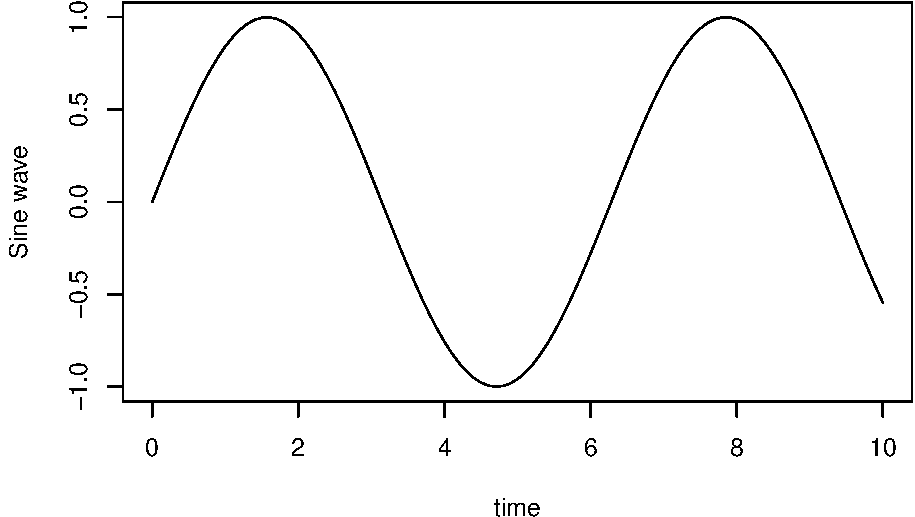
\includegraphics[width=\reprintcolumnwidth]{superbowlOT_files/figure-latex/Figure2} \caption{A sine wave.}\label{fig:Figure2}
\end{figure}

\hypertarget{inline-and-display-math-samples}{%
\section{Inline and display math
samples}\label{inline-and-display-math-samples}}

You can also include inline math, like \(\sum\nolimits_{i=1}^N a_i\).

The following is a matrix.

\[
A_{m,n} = 
 \begin{pmatrix}
  a_{1,1} & a_{1,2} & \cdots & a_{1,n} \\
  a_{2,1} & a_{2,2} & \cdots & a_{2,n} \\
  \vdots  & \vdots  & \ddots & \vdots  \\
  a_{m,1} & a_{m,2} & \cdots & a_{m,n} 
 \end{pmatrix}
\]

\hypertarget{citations}{%
\section{Citations}\label{citations}}

The code \texttt{{[}@key{]}} should usually be used for making citations
surrounded by parentheses, where \texttt{key} is the BibTeX cite-key. If
you need only the year in parentheses, you may use \texttt{@key}.

Some examples:

\begin{itemize}
\item
  Normal journal cite: \citep{joursamp1}
\item
  Volume number with issue number: \citep{joursamp3}
\item
  Journal article published online, not yet printed: \citep[published
  online,][]{sampMisc2}
\item
  Book reference: \citep{booksamp1}
\item
  In press: \citep[in press,][]{inpress2}
\item
  Website: \citep{websiteauthyear}
\item
  Inproceedings: \citep{sampinproceedings3}.
\end{itemize}

\begin{acknowledgments}
This research was supported by \ldots{}

\end{acknowledgments}

\appendix

To start the appendix, use the \texttt{\textbackslash{}appendix}
command. This signals that all following section commands refer to
appendixes instead of regular sections. Therefore, the
\texttt{\textbackslash{}appendix} command should be used only once---to
set up the section commands to act as appendices. Thereafter normal
section commands are used. The heading for a section can be left empty.
For example,

\begin{Shaded}
\begin{Highlighting}[]
\FunctionTok{\textbackslash{}appendix}

\NormalTok{\# }
\end{Highlighting}
\end{Shaded}

will produce an appendix heading that says ``APPENDIX A'' and

\begin{Shaded}
\begin{Highlighting}[]
\FunctionTok{\textbackslash{}appendix}

\NormalTok{\# Background}
\end{Highlighting}
\end{Shaded}

will produce an appendix heading that says ``APPENDIX A: BACKGROUND''
(note that the colon is set automatically).

If there is only one appendix, then the letter ``A'' should not appear.
This is suppressed by using the star version of the appendix command
(\texttt{\textbackslash{}appendix*} in the place of
\texttt{\textbackslash{}appendix}).

\hypertarget{a-little-more-on-appendices}{%
\section{A little more on
appendices}\label{a-little-more-on-appendices}}

Observe that this appendix was started by using

\begin{Shaded}
\begin{Highlighting}[]
\FunctionTok{\# A little more on appendices}
\end{Highlighting}
\end{Shaded}

Note the equation number in an appendix:

\[E=mc^2\]

% -------------------------------------------------------------------------------------------------------------------
%   Appendix  (optional)

%\appendix
%\section{Appendix title}

%If only one appendix, please use
%\appendix*
%\section{Appendix title}


%=======================================================

%Use \bibliography{<name of your .bib file>}+
%to make your bibliography with BibTeX.

%=======================================================

\bibliography{sampbib.bib}


\end{document}
